%%%%%%%%%%%%%%%%%%%%%%%%%%%%%%%%%%%%%%%%%
% Journal Article
% LaTeX Template
% Version 1.3 (9/9/13)
%
% This template has been downloaded from:
% http://www.LaTeXTemplates.com
% http://en.wikibooks.org/wiki/LaTeX/Mathematics
% Original author:
% Frits Wenneker (http://www.howtotex.com)
%
% License:
% CC BY-NC-SA 3.0 (http://creativecommons.org/licenses/by-nc-sa/3.0/)
%
%%%%%%%%%%%%%%%%%%%%%%%%%%%%%%%%%%%%%%%%%

%----------------------------------------------------------------------------------------
%	PACKAGES AND OTHER DOCUMENT CONFIGURATIONS
%----------------------------------------------------------------------------------------

%\documentclass[twoside]{article}
\documentclass[a4paper,12pt]{article}

%\usepackage{lipsum} % Package to generate dummy text throughout this template
\usepackage{mathtools} % package fixes some amsmath quirks and adds some useful settings, symbols, and environments to amsmath
\usepackage[sc]{mathpazo} % Use the Palatino font
\usepackage[T1]{fontenc} % Use 8-bit encoding that has 256 glyphs
\linespread{1.05} % Line spacing - Palatino needs more space between lines
\usepackage{microtype} % Slightly tweak font spacing for aesthetics

\usepackage[hmarginratio=1:1,top=32mm,columnsep=20pt]{geometry} % Document margins
%\usepackage{multicol} % Used for the two-column layout of the document
\usepackage{multirow}
\usepackage[hang, small,labelfont=bf,up,textfont=it,up]{caption} % Custom captions under/above floats in tables or figures
\usepackage{booktabs} % Horizontal rules in tables
\usepackage{float} % Required for tables and figures in the multi-column environment - they need to be placed in specific locations with the [H] (e.g. \begin{table}[H])
\usepackage{hyperref} % For hyperlinks in the PDF

\usepackage{lettrine} % The lettrine is the first enlarged letter at the beginning of the text
\usepackage{paralist} % Used for the compactitem environment which makes bullet points with less space between them

\usepackage{cite}
%\usepackage[numbers,sort&compress]{natbib}
%\usepackage[style=numeric]{biblatex}
%\addbibresource{thomastsai.bib}
%\bibliographystyle{ieeetr}

\usepackage{abstract} % Allows abstract customization
\renewcommand{\abstractnamefont}{\normalfont\bfseries} % Set the "Abstract" text to bold
\renewcommand{\abstracttextfont}{\normalfont\small\itshape} % Set the abstract itself to small italic text

%http://en.wikibooks.org/wiki/LaTeX/Floats,_Figures_and_Captions
\usepackage{graphicx}
%\usepackage{epsfig}
\usepackage{subcaption}
\graphicspath{ {dft/} }
\DeclareGraphicsExtensions{.pdf,.png,.jpg}

\usepackage{fancyhdr} % Headers and footers
\pagestyle{fancy} % All pages have headers and footers
\fancyhead{} % Blank out the default header
\fancyfoot{} % Blank out the default footer
%\fancyhead[C]{Running title $\bullet$ October 2014 $\bullet$ Vol. XXI, No. 1} % Custom header text
%\fancyfoot[RO,LE]{\thepage} % Custom footer text

\usepackage{pgfplots}
\pgfplotsset{compat=newest}

%\usepackage[]{algorithm2e}
\usepackage{algorithm}
%\usepackage{algorithmicx}
\usepackage{algpseudocode}
\renewcommand{\algorithmicrequire}{\textbf{Input:}}  % Use Input in the format of Algorithm
\renewcommand{\algorithmicensure}{\textbf{Output:}} % Use Output in the format of Algorithm

%\usepackage{titlesec} % Allows customization of titles
%\renewcommand\thesection{\Roman{section}} % Roman numerals for the sections
%\renewcommand\thesubsection{\Roman{subsection}} % Roman numerals for subsections
%\titleformat{\section}[block]{\large\scshape\centering}{\thesection.}{1em}{} % Change the look of the section titles
%\titleformat{\subsection}[block]{\large}{\thesubsection.}{1em}{} % Change the look of the section titles

\newtheorem{theorem}{Theorem}

%----------------------------------------------------------------------------------------
%	TITLE SECTION
%----------------------------------------------------------------------------------------

\title{\vspace{-15mm}\fontsize{24pt}{10pt}\selectfont\textbf{Study Report: Object Detection with Pixel Intensity Comparisons Organized in Decision Trees}} % Article title

\author{
\large
\textsc{Thomas Tsai}\thanks{Thomas Tsai is a RD VP in biotrump inc.}\\[2mm] % Your name
\normalsize www.biotrump.com \\ % Your institution
\normalsize \href{mailto:thomas@biotrump.com}{thomas@biotrump.com} % Your email address
\vspace{-5mm}
}
\date{}

%----------------------------------------------------------------------------------------
\def\BState{\State\hskip-\ALG@thistlm}

\begin{document}

\maketitle % Insert title

%\thispagestyle{fancy} % All pages have headers and footers

%----------------------------------------------------------------------------------------
%	ABSTRACT
%----------------------------------------------------------------------------------------

\begin{abstract}

%\noindent \lipsum[1] % Dummy abstract text
Pixel intensity comparison binary test. \cite{DBLP:journals/corr/abs-1305-4537} Decision Tree.

\end{abstract}

%----------------------------------------------------------------------------------------
%	ARTICLE CONTENTS
%----------------------------------------------------------------------------------------

%\begin{multicols}{2} % Two-column layout throughout the main article text
%\end{multicols}
%\onecolumn

\section{Introduction}
\lettrine[nindent=0em,lines=2]{I}\ am trying to list all the possible proofs.

\section{Weighted Mean Squared Error: WMSE}
A training data is a set $\{(I_s,v_s,w_s) : s=1,2,..,S\}$
where $v_s$ is the \textbf{ground truth value} associated with image $I_s$ and $w_s$ is its weight.
\\ A pixel intensity comparison binary test on a image I is defined as

\begin{equation}
\label{eq:bintest}
    bintest(I;l_1,l_2)=
\begin{cases}
    0,		& \text{if} I(l_1)\leq I(l_2)\\
    1,      & \text{otherwise}
\end{cases}
\end{equation}\\
\\ A \textbf{bintest}, $f_i$, has \textbf{only two values: 0 or 1}, so a image will be classified as 0 or 1 by the \textbf{bintest}. If an image is classified to "0", it's in class/cluster $C_0$, otherwise it's in class/cluster $C_1$. \\
\\ Scalar $\bar{v_0}$ and $\bar{v_1}$ are \textbf{weighted averages of the ground truths} in $C_0$ and $C_1$, respectively.

\begin{equation}
\label{eq:WAGT0}
\bar{v_0}=\frac{\sum\nolimits_{(I,v,w) \in C_0} w_i v_i} { \sum\nolimits_{(I,v,w) \in C_0} w_i} =
\end{equation}
\[
\frac{\sum_{i=1}^{\| C_0 \|}  w_i v_i}
{\sum_{i=1}^{\| C_0 \|}  w_i}
\]

Let $\| C_{0} \|=n$.\\
\[
\bar{v_0}=\frac{\sum_{i=1}^{\| C_0 \|}  w_i v_i}
{\sum_{i=1}^{\| C_0 \|}  w_i}=\\
\]

\begin{equation}
\label{eq:WAGT0-1}
\frac{\sum_{i=1}^{n}  w_i v_i}
{\sum_{i=1}^{n}  w_i}
\end{equation}
\\

Let $\| C_{1} \|=m$.\\
\begin{equation}
\label{eq:WAGT1}
\bar{v_1}=\frac{\sum\nolimits_{(I,v,w) \in C_1} w_i v_i} { \sum\nolimits_{(I,v,w) \in C_1} w_i} =
\frac{\sum_{i=1}^{\| C_1 \|}  w_i v_i}
{\sum_{i=1}^{\| C_1 \|}  w_i}=\\
\frac{\sum_{i=1}^{m}  w_i v_i}
{\sum_{i=1}^{m}  w_i}
\end{equation}
\\

\begin{equation}
\label{eq:WMSE}
\text{WMSE}=\text{WMSE0} + \text{WMSE1}=
\sum\nolimits_{(I,v,w) \in C_0} w (v-\bar{v_0})^2 +
\sum\nolimits_{(I,v,w) \in C_1} w (v-\bar{v_0})^2
\end{equation}
Why not variance of the C0 and C1 as the error?

\[\text{WMSE0}=\sum_{(I,v,w) \in C_0} w (v-\bar{v_0})^2=\sum_{i=1}^{\| C_0 \|} w_i (v_i - \bar{v_0})^2=
\sum_{i=1}^{\| C_0 \|} w_i (v_i^2 - 2v_i \bar{v_0} + \bar{v_0}^2)=\]

\[\sum_{i=1}^{n} w_i v_i^2 - 2\bar{v_0}\sum_{i=1}^{n} w_i v_i +
\bar{v_0}^2\sum_{i=1}^{n} w_i=\]

\[\sum_{i=1}^{n} w_i v_i^2 - 2\bar{v_0} (\bar{v_0} \cdot \sum_{i=1}^n w_i) +
\bar{v_0}^2\sum_{i=1}^{n} w_i=\]

\[\sum_{i=1}^{n} w_i v_i^2 - 2\bar{v_0} \bar{v_0} \cdot \sum_{i=1}^n w_i
+ \bar{v_0}^2\sum_i^n w_i=\]

\[\sum_{i=1}^{n} w_i v_i^2 - 2\bar{v_0}^2 \sum_{i=1}^n w_i  +
\bar{v_0}^2 \sum_{i=1}^n w_i=\]

\[\sum_{i=1}^{n} w_i v_i^2 - \bar{v_0}^2 \sum_{i=1}^n w_i = \]
\\
Refer to \eqref{eq:WAGT0-1}:
\[\sum_{i=1}^{n} w_i v_i^2 - (\frac{\sum_{i=1}^{n}  w_i v_i}
{\sum_{i=1}^{n}  w_i})^2 \sum_{i=1}^n w_i = \]

\begin{equation}
\label{eq:WMSE00}
\sum_{i=1}^{n} w_i v_i^2 - \frac{(\sum_{i=1}^{n} w_i v_i)^2}
{\sum_{i=1}^{n}  w_i} = WMSE0
\end{equation}

\begin{equation}
\label{eq:WMSE1}
\sum_{i=1}^{m} w_i v_i^2 - \frac{(\sum_{i=1}^{m} w_i v_i)^2}
{\sum_{i=1}^{m}  w_i} = WMSE1
\end{equation}


If we limit the depth of the tree to D and we consider
B binary tests at each internal node, the training time is
$O(D \cdot B \cdot S)$ for a training set containing S samples, i.e., it
is linear in all relevant parameters. This follows from the
observation that each training sample is tested with B pixel
intensity comparisons for each internal node it visits on its
path of length D from the root node to its terminal node. A
constructed tree needs $O(2^D)$ bytes for storage and its runtime
speed scales as O(D).

\section{An ensemble of trees for binary classification}
We use the \textbf{GentleBoost} algorithm \cite{Friedman98additivelogistic}, a modification of the better known \textbf{real AdaBoost}, to generate a discriminative ensemble by sequentially fitting a decision tree to an appropriate least squares problem.
We can also use \textbf{Modest AdaBoost} which produces less generalization error compared to mentioned algorithms at the cost of somewhat higher training error. \cite{GML327}

In order to generate an ensemble of K trees from a training set, the algorithm proceeds in the
following steps:

\subsection{AdaBoost Algorithms}
discrete adaboost, real adaboost, gentle adaboost, modest adaboost

\begin{algorithm}[htb]
  \caption{ AdaBoost Algorithm}
  \label{alg:adaboost}
  \begin{algorithmic}[1]
    \Require
      The set of positive samples for current batch, $P_n$;
      The set of unlabelled samples for current batch, $U_n$;
      Ensemble of classifiers on former batches, $E_{n-1}$;
    \State Extracting the set of reliable negative and/or positive samples $T_n$ from $U_n$ with help of $P_n$;
    \label{code:fram:extract}
    \State Training ensemble of classifiers $E$ on $T_n \cup P_n$, with help of data in former batches;
    \label{code:fram:trainbase}
    \State $E_n=E_{n-1}cup E$;
    \label{code:fram:add}
    \State Classifying samples in $U_n-T_n$ by $E_n$;
    \label{code:fram:classify}
    \State Deleting some weak classifiers in $E_n$ so as to keep the capacity of $E_n$;
    \label{code:fram:select} \\
    \Return $E_n$;
    \Ensure
      Ensemble Trees ;
  \end{algorithmic}
\end{algorithm}


\begin{algorithm}[htb]
  \caption{ Gentle AdaBoost}
  \label{alg:GentleAdaBoost}
  \begin{algorithmic}[1]
    \Require
	In order to generate an ensemble of \textbf{\textit{T}} trees from a training set 	$\textbf{\textit{D}}=\left\{ { (I_s,c_s) | s=1,2,3,...,S}\right\}$. Where $I_s$ is the input image and $c_s$ is the class label. $c_s \in \left\{{-1,+1 } \right\}$. -1 is a non-face sample image and +1 is a face sample image.
    \State Initialize the weight $w_s$ for each image $I_s$ and its class label $c_s \in
    	\left\{ {+1,-1}\right\}$ as:

    $w_s=
	\begin{cases}
    1/P,	& c_s = +1 \\
    1/N,    & c_s = -1
	\end{cases}$

		Where \textbf{P} is the total number of positive samples, $c_s=+1$, and \textbf{N} is the total number
		of negative samples, $c_s=-1$.
    \State For $k = 1,2,...,K:$
    \begin{itemize}
	\item[a.]{\textbf{Find/Fit} a decision tree $T_k$ by weighted least squares of $c_s$ to $I_s$ with
	weights $w_s$}. Refer to equation \eqref{eq:WMSE_01}.
	\item[b.]{Update weights:}\\
		$w_{s,k+1} = w_{s,k} \cdot \exp^{-c_s T_k(I_s)}$\\
		where $T_k(I_s)$ denotes the \textbf{real-valued} output of a regression tree $T_k$ on image $I_s$.
	\item[c.]{Renormalize weights, $w_{s,k+1}$ , so they sum to 1.}
	\end{itemize}
    \Ensure
      Ensemble of classifiers/trees $\left\{ { T_k | k=1,2,3,...,K}\right\}$.
  \end{algorithmic}
\end{algorithm}

\begin{algorithm}[htb]
  \caption{ Modest AdaBoost}\cite{GML327}
  \label{alg:ModestAdaBoost}
  \begin{algorithmic}[1]
    \Require
	In order to generate an ensemble of \textbf{\textit{T}} trees from a training set 	$\textbf{\textit{D}}=\left\{ { (I_s,c_s) | s=1,2,3,...,S}\right\}$. Where $I_s$ is the input image and $c_s$ is the class label. $c_s \in \left\{{-1,+1 } \right\}$. -1 is a non-face sample image and +1 is a face sample image.
    \State Initialize the weight $w_s$ for each image $I_s$ and its class label $c_s \in
    	\left\{ {+1,-1}\right\}$ as:

    $w_s=
	\begin{cases}
    1/P,	& c_s = +1 \\
    1/N,    & c_s = -1
	\end{cases}$

		Where P is the total number of positive samples, $c_s=+1$, and N is the total number of negative samples , 			$c_s=-1$.
    \State For $k = 1,2,...,K:$
    \begin{itemize}
	\item[a.]{\textbf{Find/Fit} a decision tree $T_k$ by weighted least squares of $c_s$ to $I_s$ with
	weights $w_s$}. Refer to equation \eqref{eq:WMSE_01}.
	\item[b.]{Update weights:}\\
		$w_{s,k+1} = w_{s,k} \cdot \exp^{-c_s T_k(I_s)}$\\
		where $T_k(I_s)$ denotes the real-valued output of tree $T_k$ on image $I_s$.
	\item[c.]{Renormalize weights so they sum to 1.}
	\end{itemize}
    \Ensure
      Ensemble of classifiers/trees $\left\{ { T_k | k=1,2,3,...,K}\right\}$.
  \end{algorithmic}
\end{algorithm}

\section{Sensitivity to noise}
\begin{figure}[ht]
  \centering
  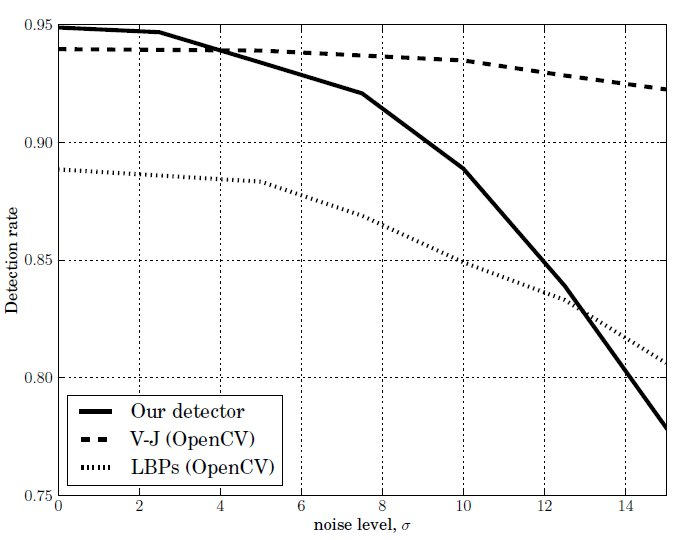
\includegraphics[width=\textwidth, keepaspectratio=true]{ObjectDetectionPixelIntensityFig6-.jpg}
  \caption{Detection rate on the GENKI-SZSL dataset for different noise levels.}
 \label{fig:fig6}
\end{figure}

\begin{figure}[h!]
  \centering
  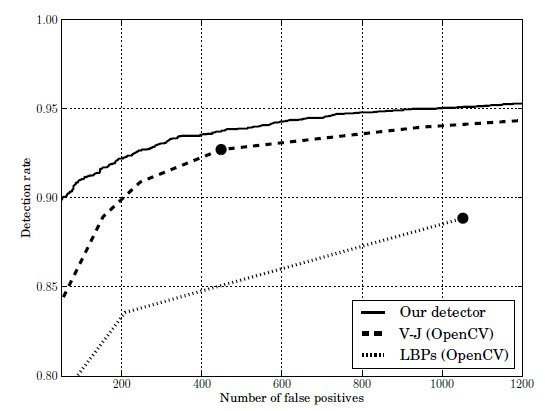
\includegraphics[width=\textwidth, keepaspectratio=true]{ObjectDetectionPixelIntensityFig2.jpg}
  \caption{ROC curves for the GENKI-SZSL/NO-FACES-1 experiment.}
 \label{fig:fig2}
\end{figure}


\begin{figure}[h!]
  \centering
  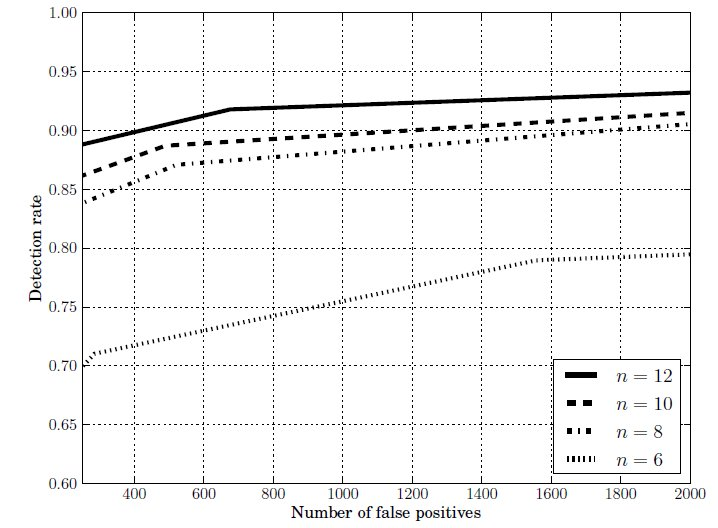
\includegraphics[width=\textwidth, keepaspectratio=true]{ObjectDetectionPixelIntensityFig7.jpg}
  \caption{ROC curves for different number of considered face orientations, n, during the scan of each image.}
 \label{fig:fig7}
\end{figure}

This method performs \textbf{poor} in the presence of \textbf{high noise levels} due to
\textbf{simplicity of the used binary tests}. The features used by OpenCV detectors should be robust in these circumstances as they are based on \textbf{region averaging}, which corresponds to \textbf{low--pass filtering}.

We use the \textbf{additive (uncorrelated) Gaussian noise model} to \textbf{quantitatively} evaluate these effects:
A sample from a Gaussian distribution with \textbf{zero mean} and \textbf{standard deviation} is added to the intensity of each image pixel.

An experiment on the GENKI-SZSL dataset is reported in \autoref{fig:fig6}. We see that the \textbf{detection rate of our system degrades significantly as the noise intensity increases}. These adverse effects can be reduced by applying a \textbf{low-pass filter prior to detection}.
\textbf{This is not necessary as the noise levels in this experiment are uncommon for modern cameras,
even on mobile devices.}

The images in the GENKI-SZSL dataset are already \textbf{noisy} and contain
\textbf{compression artefacts}, i.e., they are representative of the ones encountered in real world
face detection applications.

The other systems based on similar features could be sensitive to high noise levels as well. An example of such a commercial system is the Microsoft Kinect human pose recognizer, described in

\section{Detecting rotated faces}
A simple solution of the object detection under \textbf{general planar rotations} is to scan the
image at \textbf{multiple orientations}. In our case, this can be performed
\textbf{without image resampling} as pixel intensity comparison binary tests can be easily rotated for a given angle (in our implementation, we use \textbf{precomputed look-up tables} as this
proved faster than evaluating trigonometric functions at runtime).
It is not immediately clear if this leads to acceptable
performance since it could result in poor processing speeds and/or large number of false positives.

We use the \textbf{previously learned face detector} and provide experimental analysis.
To investigate the \textbf{detection accuracy}, we \textbf{rotate each image} found in the GENKI-SZSL dataset
for a \textbf{random angle} sampled uniformly from the $[0, 2\pi]$ interval.
We report \textbf{false positives} on the NO-FACES-1 set. Results can be seen in \autoref{fig:fig7}.

By comparing the \textbf{ROC curves} to the ones in \autoref{fig:fig2},
we can see that the accuracy of the approach is comparable to the OpenCV's LBP-based frontal face detector.

%http://www.tablesgenerator.com/
\begin{table}[hb]
\begin{tabular}{|l|l|l|l|l|}
\hline
\multirow{2}{*}{Device} & \multicolumn{4}{l|}{Time {[}ms{]}} \\ \cline{2-5}
                        & n = 6   & n=8    & n=10   & n=12   \\ \hline
PC1                     & 15.8    & 20.6   & 25.8   & 31.2   \\ \hline
PC2                     & 21.6    & 26.8   & 34.5   & 42.9   \\ \hline
\end{tabular}
\caption{Average times required to process a 640x480 pixel image at n orientations, attempting to find faces larger than 100 x 100 pixels at all possible planar rotations}
\label{tab:table3}
\end{table}

Processing speeds can be seen in \autoref{tab:table3}. These results demonstrate
that our system can perform \textbf{rotation invariant} face detection
with reasonable accuracy in \textbf{real-time} using a \textbf{single core} of a modern personal computer.

\section{Qualitative results}
A video demonstrating \textbf{rotation invariant} face detection is available at
\url{http://youtu.be/1lXfm-PZz0Q}.
Furthermore, demo applications can be downloaded from \url{http://public.tel.fer.hr/odet/}.
\textbf{Complete source code} is provided at \url{https://github.com/nenadmarkus/pico}.

\section{Conclusion}
An object detection system based on pixel intensity comparisons organized in decision trees
can achieve competitive results at high processing speed. This is especially evident on devices with limited hardware support for floating point operations. This could prove important in the embedded system and mobile device industries because it can reduce hardware workload and prolong battery life.
Further advantages of our method are:
\begin{compactitem}
\item The method does not require the computation of integral
images, image pyramid, HOG pyramid or any other
similar data structure.
\item All binary tests in internal nodes of the trees are based on
the same feature type. For comparison, Viola and Jones
used 5 different types of Haar-like features to achieve
their results.
\item There is \textbf{no need for image preprocessing prior to detection} (such as contrast normalization, resizing, Gaussian smoothing or gamma correction).
\item The method can easily be modified for fast detection of \textbf{in-plane rotated} objects.
\end{compactitem}

%----------------------------------------------------------------------------------------
%	REFERENCE LIST
%----------------------------------------------------------------------------------------
\clearpage
%\printbibliography
%\bibliography{abbr_long,pubext}
\bibliography{thomastsai.bib}{}
\bibliographystyle{ieeetr}

%\begin{thebibliography}{99} % Bibliography - this is intentionally simple in this template

%\bibitem[Figueredo and Wolf, 2009]{Figueredo:2009dg}
%Figueredo, A.~J. and Wolf, P. S.~A. (2009).
%\newblock Assortative pairing and life history strategy - a cross-cultural
%  study.
%\newblock {\em Human Nature}, 20:317--330.

%\end{thebibliography}

%----------------------------------------------------------------------------------------

%\end{multicols}

\end{document}
